% Use a modified ACM conference proceedings template
\documentclass[sigconf]{acmart}
% Disable some elements from ACM template
\setcopyright{none}
\settopmatter{printacmref=false,printfolios=false}

\usepackage{booktabs} % For formal tables
\usepackage[ruled,vlined]{algorithm2e}
\usepackage{amsmath} % for writing algorithms
\usepackage{cleveref}
\usepackage{subcaption}
\usepackage{listings}

% OWN COMMANDS
\newcommand{\todo}[1]{{\color{red}{#1}}}

% VARIABLES
\usepackage{xspace} % allows \commmand instead of \command{} with correct space afterwards
\newcommand{\VNumSimulations}{20\xspace}
\newcommand{\VNumDays}{10.000\xspace}
\newcommand{\VNumPop}{100\xspace}
\newcommand{\VNumTrees}{140\xspace}
\newcommand{\VProbPredator}{0.003\xspace}
\newcommand{\VProbAltruistDies}{0.50\xspace}
\newcommand{\VProbKids}{0.001\xspace}


\newcommand{\cowards}{\textit{cowards}\xspace}
\newcommand{\coward}{\textit{coward}\xspace}
\newcommand{\altruist}{\textit{altruist}\xspace}
\newcommand{\altruists}{\textit{altruists}\xspace}
\newcommand{\suckers}{\textit{suckers}\xspace}
\newcommand{\sucker}{\textit{sucker}\xspace}
\newcommand{\impostors}{\textit{impostors}\xspace}
\newcommand{\impostor}{\textit{impostor}\xspace}
\newcommand{\greenbeards}{\textit{greenbeards}\xspace}
\newcommand{\greenbeard}{\textit{greenbeard}\xspace}


\begin{document}
    \title{On Trust and Prosociality}

    \author{Fatjon Zogaj}\affiliation{}
    \email{fzogaj@student.ethz.ch}

    \author{Rafael Sterzinger}\affiliation{}
    \email{rsterzinger@student.ethz.ch}

    \begin{abstract}
        The concept of fitness and its connotation to survival in the evolutionary sense lead to the emergence of deflection and cooperation-based strategies.
        Conducting a variety of experiments, we analyze the notions of altruism and trust, based on varying levels of (mis)information.
        We show that altruism itself affects population size positively in both true (selfless) and fair (reciprocal) cases.
        With the introduction of misinformation the effectiveness of cooperation decreases substantially.
        As such honesty and trust are key components in societal populations as even with small amounts of deception, altruistic behaviour goes extinct.
        %\todo{Briefly summarize your report here. This should include a description of the task you are solving, a summary of how you approach the task (i.e. your method), as well as a preview of the central result. The abstract should be short, i.e. 4-5 sentences. The rest of this template outlines a rough structure how you \emph{can} organize your report. It mentions all the components we would typically expect. It is a good idea to adhere these guidelines, but they are not binding, i.e., you are free to re-organize your report as you see fit.}
        %\todo{check bibliography}
        %\todo{check numbers of changed plots}
    \end{abstract}

    \maketitle


    \section{Introduction}\label{sec:introduction}
    %In this section, introduce the task in a bit more detail. In the first paragraph, try to answer why the task is of interest at all and what makes it challenging. You may also discuss some related work here. For example, you can summarize how other researchers have addressed the problem and what might be the disadvantages of these works.


    The evolution of cooperation is a question which has been bothering humanity for a long time.
    Not only is it open for debate in the fields of anthropology, sociology and economy, also evolutionary biologist have tried to answer this question on multiple occasions~\cite{gardner_theory_2009}.
    Hence, in 2005, at the 125th anniversary issue of the American Association for the Advancement of Science (AAAS), they declared the question "How Did Cooperative Behavior Evolve?" to be one of the top 25 unsolved puzzles on which science should focus over the next quarter century~\cite{aaas_125th_2005}.

    Already in the year~\citeyear{darwin_origin_1859}, \citeauthor{darwin_origin_1859}'s natural selection theory tried to explain the underlying mechanisms of a growing population.
    More helpful characteristics that lead to better reproduction will keep on spreading throughout the population \cite{darwin_origin_1859}.
    This gives off the impression that certain traits will develop in order to optimize an individual's reproducibility (fitness). \citeauthor{fisherGeneticalTheoryNatural1930} \cite{fisherGeneticalTheoryNatural1930} builds upon this by introducing the notion of gene frequencies.
    Genes leading to higher individual fitness thus will increase in frequency and lead to a general increase in mean fitness.


    %In the second half of the introduction, describe your method. This should be more detailed than in the abstract. You can talk about how your method relates to existing work (e.g. it is a combination or extension of existing methods, what other papers were you inspired by, etc.). You should also state the central result here, and the key insight that made it possible to achieve this result.

    Based on this idea of fitness, different survival strategies can occur in nature, for instance, there are as many games where cooperative strategies succeed as ones where deflection performs better.
    Being heavily influenced by the amount of information an agent has over another \cite{wallace_misinformation_1973}, in our work, we want to add an additional layer of difficulty by introducing the possibility of spreading misinformation.
    Here, the goal is that misinformation might give an agent a distorted perception on the behaviour of other kinds, i.e. resulting in the existence of so-called \impostors (see \Cref{sec:hypothesis}).
    Similar research has previously been conducted, with the closest being the work by \citeauthor{szamado_deception_2016} \cite{szamado_deception_2016} where they looked at the influence of noisy gossip on cooperative behaviour in an indirect reciprocity setting via image scoring (see \Cref{sec:related_work}).
    As opposed to our work, agents can adaptively change their reputation by being more cooperatively, whereas we explore the idea of misinformation from a more static point of view, that is, an agent decides and shares from the beginning onwards whether it wants to cooperate but might not do this in disguise.

    For this, we conduct a variety of experiments to analyze how different levels of cooperation and environment settings affect a population and the development of respective types/tribes within.
    With these simulations, we seek to provide a profound answer to the question on whether it is possible for cooperative behaviour to co-exist in reputation based settings where misinformation gives rise to disguised cheats.

    These simulations consist of \VNumSimulations runs, each spanning \VNumDays days where we visualize and analyze the average results of those runs.
    The general environment looks as follows: based on a starting population of \VNumPop, these starting agents compete for $2 \times \VNumTrees$ possible jobs to earn money every day.
    Furthermore, one or two agents are assigned to a department where they work on their individual task resulting in \VNumTrees overall departments.
    To simplify the case, we say that if an agent is not able to win any of the $2 \times \VNumTrees$ job options, he goes bankrupt and dies out, hence limiting the total population size.
    On top of that, not every one of the jobs is a guaranteed win.
    With a certain probability of \VProbPredator a job is considered to be difficult and if only one agent has taken on that job, he dies out.
    Here, the possibility of cooperation arises: if an agent with a normal job decides to help an agent with a difficult job from its department, the agent who was previously doomed to die will survive.
    However, this comes at the risk that the previously safe agent might not be able to finish its task on time and, thus might go bankrupt itself.
    We say that with a certain probability of \VProbAltruistDies the helping agent fails and ends up sacrificing itself for the other.


    \begin{enumerate}
        \item In our first experiment we create a stable environment so that the population stays roughly the same.
        Therefore, agents are not able to split a difficult job between each other.

        \item Next, we introduce altruistic thinking.
        As such, an altruist (later called \sucker) always tries to help out an agent assigned with a difficult job.
        By doing so, the other agent is able to live on while the helping altruist now has the burden of doing both job options with the possibility of failing its original one and thus dying.

        \item Building upon the previous experiment, we introduce a fairer notion where altruists turn into \greenbeards that only help out other \greenbeards.
        Thus, they ignore uncooperative agents that do not bear the green beard allele.

        \item A final experiment introduces further types next to the altruist/\greenbeard.
        The final types are as follows: \cowards (never help with difficult jobs), \suckers (always help with difficult jobs), \impostors (look like \greenbeards, but never help) and \greenbeards (only help other bearers of the green beard allele, aka \impostors and \greenbeards).
        Here, the portion of \impostors act as a resemblance of misinformation spread in a population, i.e. the more \impostors there are, the more the \greenbeards obtain deceptive information.

    \end{enumerate}

    We analyze these cases with a variety of different parameters which are explained in further detail in \Cref{sec:method} and \Cref{sec:evaluation}, and can be inspected in \Cref{sec:configs}.


    Going further, we provide a general taxonomy on the basis of cooperative behaviour, starting with inclusive fitness, followed by the more granular distinction between direct and indirect fitness.
    This is then followed by a section focusing on indirect reciprocity which we separated from the other section in order to put more emphasise on it as this cooperative mechanism plays a key role in our research question.

    Through our experiments we show that honesty and trust are key components for large-scale human societies.
    Without this, altruism via reputation-based cooperation is an unstable phenomenon that goes extinct through the introduction of the aforementioned \impostors.


    \section{Inclusive Fitness}\label{sec:inclusive-fitness}

    Already back in the days, when \citeauthor{darwin_origin_1859} \cite{darwin_origin_1859} developed his theory on the origin of species, the idea of cooperative behaviour stood in contrast to his beliefs of natural selection and the fitness of individuals, that is the reproductive success that allows a species to dominate one another \cite{pennisi_how_2005}.
    Here, the key problem was that maximization of individual fitness does not align with the occurrence of altruistic or spiteful traits as acting cooperatively is costly and therefore would lower their own fitness level \cite{west_altruism_2010}.
    \citeauthor{darwin_origin_1859} later describes scenarios in which altruism could indirectly improve individual fitness by cooperating among kin, i.e. supporting the transmission of underlying, related genes \cite{pennisi_how_2005,gardner_theory_2009}.
    This idea was later picked up by \citeauthor{hamilton_kin_1964} \cite{hamilton_kin_1964} who has formalized \citeauthor{darwin_origin_1859}'s idea and proposed \citeauthor{hamilton_kin_1964}'s rule:

    \begin{equation}
        rb-c>0\label{eq:rb-c}
    \end{equation}


    This inequality describes in which settings a specific trait will be favored over another by natural selection.
    Here, $c$ denotes the costs of being altruistic for the actor, $b$ encapsulates the benefit of the altruistic act for the recipient, and $r$ is a measure of the genetic relatedness between the actor and the recipient \cite{west_altruism_2010}.
    This formulation is also known as inclusive fitness which is a composition of direct fitness (\Cref{subsec:direct_fit}), i.e. the improvement of individual fitness, and indirect fitness (\Cref{subsec:indirect_fitness}), i.e. enhancing the reproductive success of other genetic related individuals.
    \Cref{fig:hamilton} summarizes this composition graphically.

    Indirect fitness can most easily be observed through interactions with others of the same kin.
    Kin here refers to somebody else sharing a common trait of genes that are inherited from one common ancestor.
    Indirect fitness is often also termed \textit{kin selection} \cite{west_altruism_2010}.

    For the introduction of the different subcategories of direct and indirect fitness, we will borrow definitions from the more recent work by \citeauthor{west_altruism_2010} \cite{west_altruism_2010} instead of the work by \citeauthor{gardner_theory_2009} \cite{gardner_theory_2009}.

    \begin{figure}
        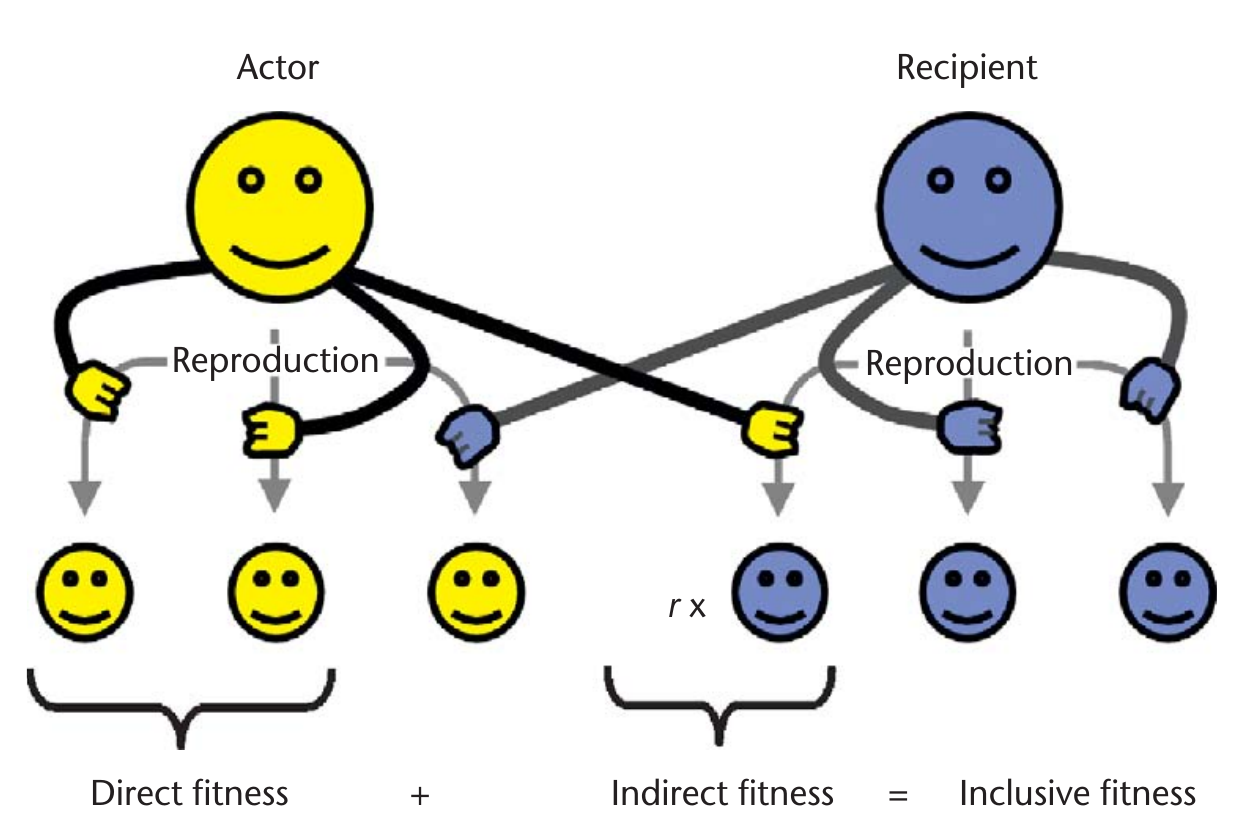
\includegraphics[width=\columnwidth]{figures/hamiltons_rule}
        \caption{\citeauthor{hamilton_kin_1964}'s rule describes inclusive fitness which consists of direct fitness $-c$ and indirect fitness $rb$ (see \Cref{eq:rb-c}). With this rule, four basic types of social behaviour can be derived \cite{gardner_theory_2009}.}
        \label{fig:hamilton}
    \end{figure}

    \subsection{Direct Fitness}\label{subsec:direct_fit}

    \subsubsection{Altruism}
    One can differentiate between two different kinds of altruism.
    The first refers to the more commonly known general case of selflessness where one helps everyone, regardless of how related they are.
    This is the case which we are analyzing in our earlier experiments, where \suckers help other \suckers and \cowards.

    The other notion of altruism refers to within-kin altruism where one only collaborates with related members of the population (see \Cref{fig:mechanisms} A).
    In our later experiments we also look at this other case by introducing the notion of \greenbeards which only help other beard-kins out.

    \subsubsection{Reciprocity}\label{reciprocity}
    Compared to regular altruism, reciprocity cannot be considered truly altruistic, as the underlying mutual benefit is based on reciprocal cooperation and not selflessness~\cite{triversEvolutionReciprocalAltruism1971} (see \Cref{fig:mechanisms} B).
    In the case where agents help others that have helped them before, cooperation leads to a direct fitness increase.
    This holds only if the short term cost $c$ is smaller than the long term benefit $b$.

    \subsection{Indirect Fitness}\label{subsec:indirect_fitness}

    \subsubsection{Spite}
    As part of inclusive fitness, the roots behind the theory of altruism can be found.
    On top of that we find a similar mechanism to altruism, that differs in its manifestation.
    Spiteful behaviour can be thought of as acts that harm the recipient (and potentially the actor).
    This way, while the harmed recipient may suffer from reduced fitness, one is able to indirectly cause an increase in fitness for other participants by removing the recipient from the pool of competition~\cite{hamiltonSelfishSpitefulBehaviour1970}.

    Looking at \Cref{eq:rb-c}, we consider the case where the relatedness factor $r$ can be negative.
    A negative value could stand for the fact that the recipient is further from the actor than the average population in relatedness.
    As such, even with a positive $c$ value (actor is harmed) and a negative $b$ value (recipient is harmed), the equation can be fulfilled.
    This, for instance, is the case where other participant that are more closely related benefit from less competition and the less related recipient gets harmed.
    Looking at \Cref{fig:mechanisms} this is visualized in \Cref{fig:mechanisms} C and can be thought of as altruism towards closer kin~\cite{west_altruism_2010}.

    From the lens of our experiments, the sort of \greenbeards we analyze, end up possessing spiteful traits by helping out their own kin (direct altruism), and letting the others die out (direct spite, indirect altruism).

    \subsubsection{Green Beard}
    Compared to the previously mentioned cases of altruism (help out everyone or help out own kin) another form of altruism can be noted.
    According to \citeauthor{hamiltonInnateSocialAptitudes1975}, for there to be indirect fitness benefits, the occurrence of the same genetic strain plays a role and not the kinship itself~\cite{hamiltonInnateSocialAptitudes1975} (see \Cref{fig:mechanisms} D).
    A certain trait or characteristic can be used to differentiate between sharers of the same gene variation and thus used to decide on whom to help.
    Natural selection here takes place in regard to that certain gene.
    To visualize this, one can think of a gene that is responsible for the growth of a green beard where those affected individuals end up cooperating between themselves~\cite{SelfishGeneRichard}.
    Note that this holds true even if the gene does not manifest itself visually, but leads to association between gene-sharers (e.g. a social gene; social people tend to stick with social people).

    An example of this green beard phenomenon occurring in nature was discovered by \citeauthor{keller_selfish_1998} \cite{keller_selfish_1998} where they found a spiteful green beard allele in the red imported fire ant species.
    Here, worker ants wearing a certain type of allele (bearer) are able to distinguish and lure queens of a different type (non-bearer) by odour cues and execute them resulting in fitness benefits for the worker ants.

    In real life this also opens up the possibility for so-called \textit{falsebeards} which do seem to have inherited the same gene from the outside, but in fact do not end up cooperating as expected.
    We analyze this case in our final experiment by introducing \impostors.

    \begin{figure}
        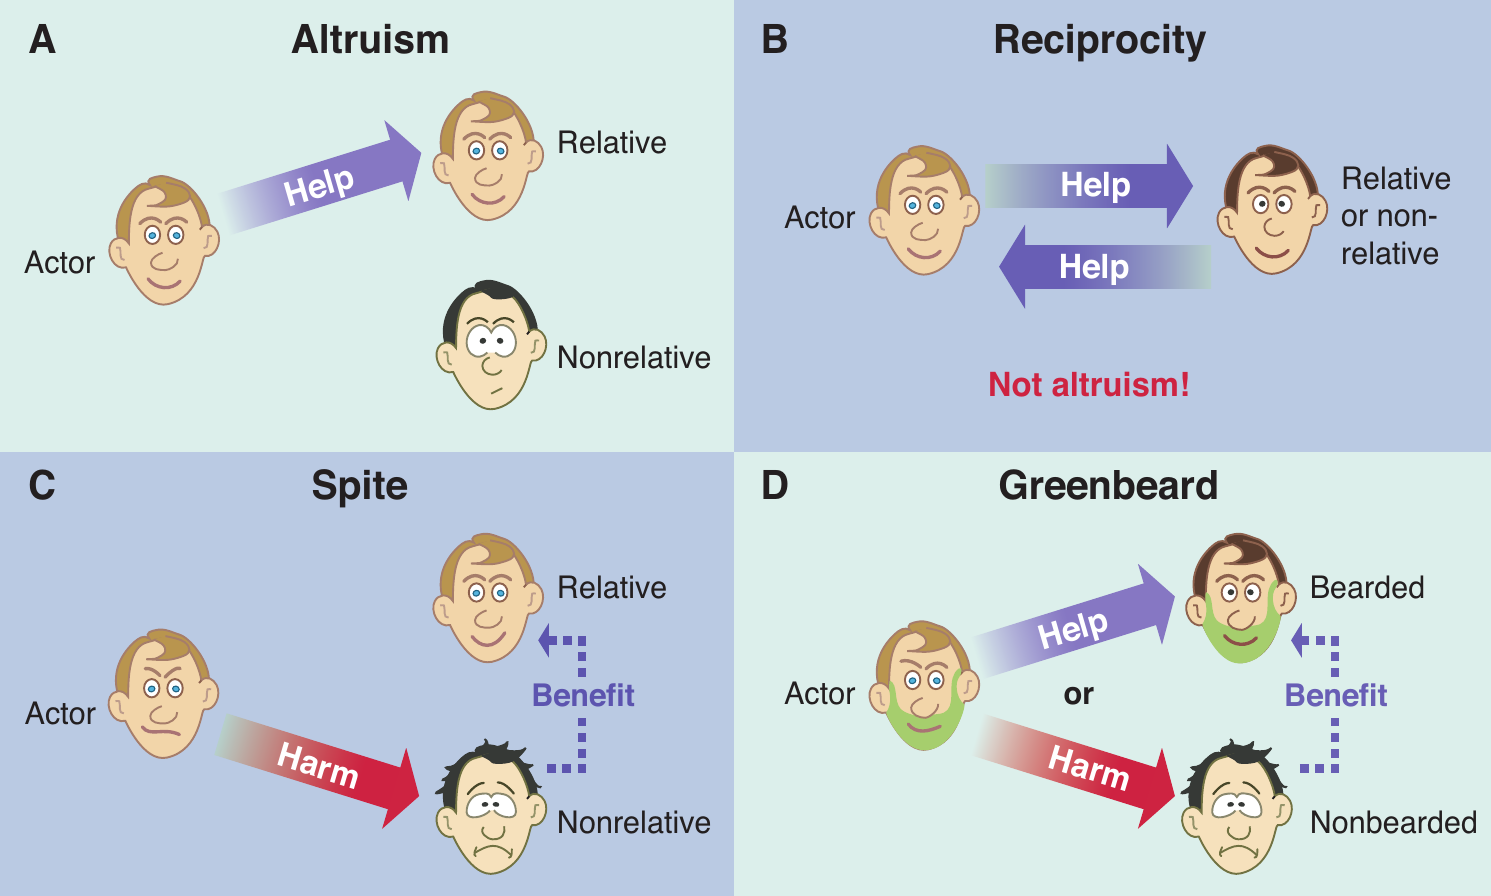
\includegraphics[width=\columnwidth]{figures/mechanisms}
        \caption{Altruism, Reciprocity, Spite, and Green Beard: The four mechanisms describe by \citeauthor{hamilton_kin_1964}'s rule \cite{west_altruism_2010}.}
        \label{fig:mechanisms}
    \end{figure}


    \section{Indirect Reciprocity}\label{sec:indirect_reciprocity}
    Another important concept is the mechanism of indirect reciprocity which is closely related to direct reciprocity (\Cref{reciprocity}), with the difference that reciprocation comes from another individual who is not the original recipient \cite{alexander_biology_1987,boyd_evolution_1989}.
    The significance of this idea stems from the fact that research beliefs that indirect reciprocity played a key role in establishing large-scale human societies \cite{roberts_kin_2019}.
    This importance initially arose when the idea of cooperative reputation, e.g. the image scoring strategy or more sophisticated mechanisms such as the standing strategy \cite{leimar_evolution_2001,ohtsuki_leading_2006}, were proposed that provided an explanation on why indirect reciprocity might work \cite{nowak_evolution_1998}.
    Here, the idea is that actors/donors base their decision of whom to donate to on a score which is based on a recipient's reputation.
    This consequently means that cooperation can occur even if the donor, and the recipient have never met.
    Different experiments conducted in the past support this phenomenon \cite{nowak_five_2006, milinski_cooperation_2002, milinski_reputation_2002,milinski_reputation_2016}.

    A very different view on the idea of indirect reciprocity provides the paper by \citeauthor{roberts_kin_2019} \cite{roberts_kin_2019} where he argues that this type of cooperation is rather driven by relatedness instead of actual reciprocity.

    "[...] individuals do not help other helpers to receive something back from third parties; instead, they help because this features the spread of a strategy of helping those who help others [...]" \cite{roberts_kin_2019}


    Concerning indirect reciprocity via image scoring, \citeauthor{roberts_kin_2019} argues that results from previously conducted experiments have been misinterpreted as evidence for indirect reciprocity.
    For instance, in an experiment by \citeauthor{milinski_reputation_2002} \cite{milinski_reputation_2002}, their result was used to explain indirect reciprocity but it lacked insights whether or not donors actually got higher payoffs by playing the image scoring strategy.
    This is a key problem as higher payoffs are a requirement for indirect reciprocity.
    Furthermore, demonstrating that an individual who plays the image scoring strategy performs better would still not be enough proof for indirect reciprocity via image scoring as self-interested players who want to maximize their own payoff would donate indiscriminately in a population dominated by image scorers as donating more results in higher payoffs \cite{roberts_kin_2019}.
    According to \citeauthor{roberts_kin_2019}, the phenomenon which actually needs to be shown is that "those who discriminate most have a higher payoff than those who give to anyone" \cite{roberts_kin_2019}.

    Regarding the idea of image scoring strategies being actually driven by relatedness, \citeauthor{roberts_kin_2019} refers back to \citeauthor{hamilton_kin_1964}'s rule.
    According to \Cref{eq:rb-c} altruism is beneficial if the benefit $b$ for the recipient, scaled by the relatedness $r$ outweighs the costs $c$ for the actor.
    Similarly, \citeauthor{nowak_five_2006} \cite{nowak_five_2006} derives an equation for indirect reciprocity via image scoring:

    \begin{equation}
        qb - c > 0\label{eq:qb-c}
    \end{equation}

    Here, $q$ denotes the so-called \textit{social acquaintanceship}, i.e. the probability of knowing the recipient's image score.
    Based on this similar notation, \citeauthor{roberts_kin_2019} argues that $q$ is actually relatedness.

    "Individuals should pay the cost of helping when this is offset by the benefit to the recipient multiplied by their chance of sharing the same strategy." \cite{roberts_kin_2019}

    Hence, altruism is selected by means of indirect fitness rather than indirect reciprocity.

    This idea of indirect reciprocity being related to kin selection is summarized in \Cref{fig:indirect_reciprocity}.

    \begin{figure*}
        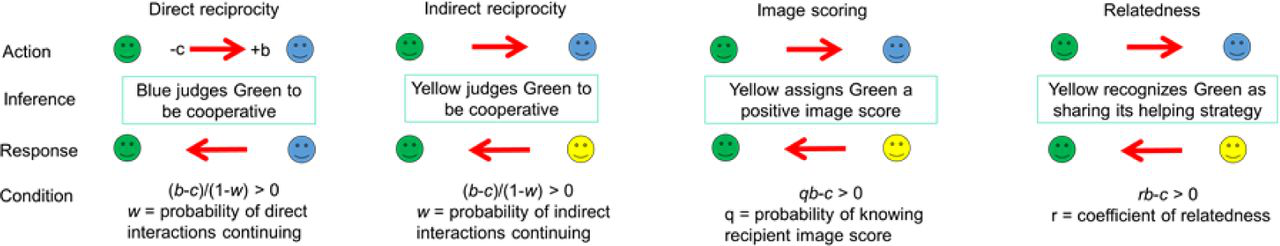
\includegraphics[width=\textwidth]{figures/indirect_reciprocity}
        \caption{The relation/similarity between direct and indirect reciprocity, and image scoring and relatedness/the green beard phenomenon \cite{roberts_kin_2019}.}
        \label{fig:indirect_reciprocity}
    \end{figure*}

    \citeauthor{roberts_kin_2019} goes even further and says that reciprocity is an illusion and that image scores an individual observes are actually cues about kinship.
    Important for our experiments is the idea that in absence of actual relatedness \greenbeards are observed that help individuals to distinguish between contributors and free riders \cite{roberts_kin_2019}.


    \section{Hypothesis}\label{sec:hypothesis}
    Inspired by the work of \citeauthor{milinski_cooperation_2002} \cite{milinski_cooperation_2002} and the additional insights from \citeauthor{roberts_kin_2019} \cite{roberts_kin_2019}, we found the idea of image scoring and how it can enforce cooperation in a public goods game without/little punishment very interesting.
    Given the idea that this image score is mostly spread via gossip in our society, we pose the question on whether this gossip can always be trusted.
    Similarly to the game "Chinese Whispers/Telephone", we argue that gossip might be altered by some noise over time resulting in a scenario where agents with an actual bad image score might be perceived as being cooperative.
    As a result from that, \impostors might occur which seem to act cooperatively influencing the overall effectiveness of cooperation.

    Based on this posed question, we want explore whether in such a setting cooperation would still outweigh defection or if defection would take over.
    We hypothesise that misinformation or deception has a major influence on the effectiveness of cooperation and that as soon as misinformation gets introduced to the setting, altruism via cooperation gets unstable quickly.
    Furthermore, we think that the amount of misinformation does not necessarily play an important role rather if misinformation exists or not.
    Based on the previously mentioned (\Cref{sec:indirect_reciprocity}) relation between indirect reciprocity and relatedness, or image scoring and the green beard phenomenon, we proceed in our experiments with \greenbeards as a means for a static image scoring mechanism.

    In order to be more concrete, we argue that the more noise is injected in $q$ from \Cref{eq:qb-c} or in other words, the more imposters are prominent, the rarer it is to observe cooperative behaviour.


    \section{Related Work}\label{sec:related_work}
    One of the first more extensive studies on information and its influence on a species' fitness was explored by \citeauthor{wallace_misinformation_1973} \cite{wallace_misinformation_1973} where he built upon the claim by \citeauthor{fisherGeneticalTheoryNatural1930} \cite{fisherGeneticalTheoryNatural1930} and proved its correctness, that is, if misinformation is spread it should highly deviate from the truth.
    He explained first why accurate information about one's environment is of great importance and that deceptive information results in a loss of the recipient's fitness and formally proved second that slightly misleading information has a probability of one half to improve the fitness of an actor.
    Hence, information must be highly misleading to be truly effective.

    As described in \Cref{sec:indirect_reciprocity}, image scoring is similar to relatedness/the green beard phenomenon which is why the concept of \textit{falsebeards} plays a significant role in our work.
    Described in multiple papers \cite{SelfishGeneRichard,roberts_kin_2019,west_altruism_2010}, the effect of cheating \textit{falsebeards} are directly responsible for the non-existence of cooperative behaviour.
    Here, a false beard describe the act where an entity disguises himself to be a bearer of a green beard allele, but is not.
    Hence, it is purposefully transmitting misinformation regarding its true intentions and thus taking advantage of the altruism of truthful green beard bearers \cite{SelfishGeneRichard}.
    For this reason, \citeauthor{SelfishGeneRichard} \cite{SelfishGeneRichard} argues that the green beard mechanism is of rare existence in nature, hinting that cooperative behaviour based on the green beard phenomenon is unstable if misinformation about the true strategy of individuals is spread.

    A more modern and very similar work to ours is the paper published by \citeauthor{szamado_deception_2016} \cite{szamado_deception_2016} where they specifically looked at how gossip mechanisms in indirect reciprocity via image scoring influences cooperation.
    They concentrated on the same idea as we did where they posed the question on how random errors during gossip or even deceptive communication give rise to the collapse of cooperation.
    Therefore, our work is complementary to theirs as we both pursue the same question, however, with a different methodological approach.
    Based on their experiments, they empirically showed that allowing the spread of deceptive information turns the image-scoring-based reputation worthless and thus cooperation is rarer or non-existing.
    Additionally, as we expect equal outcomes of our experiments, their findings act as a sanity check for our results.

    In a later work from \citeyear{whitaker_indirect_2018}, \citeauthor{whitaker_indirect_2018} \cite{whitaker_indirect_2018} looked at the evolution of prejudicial groups in indirect reciprocity interactions between actors.
    As prejudice is an opinion about other actors, not based on reason or experience, it is similar to the spread of misinformation concerning the reputation of actors belonging to another group, hence, explaining the relatedness to our work.
    With the help of computer simulations, they were able to show co-evolution of prejudicial groups and cooperative behaviour, despite the general view of those being opposing forces.
    However, prejudice restricts the ability of cooperation to flourish somehow as cooperative behaviour can solely be observed in isolated groups that have the same opinion on particular groups of outsiders.
    This shows, although being limited, that cooperation can still exist even with perturbed information or intentionally spread lies.


    \section{Method}\label{sec:method}
    This section covers our experiment setup including the different kind of parameters we vary as well as detailed explanations regarding our environment and the logic of the simulations we run.
    In general the situation can be thought of as follows.
    Based on a starting population of \VNumPop, these \VNumPop agents compete for a certain amount of limited resources.
    We cap these at \VNumTrees, but allow one such resource to be shared by two agents, leading to effectively 2~*~\VNumTrees resources.
    The reason for this is that two agents sharing a resource can help each other out in the case that part of the resource turns out to be faulty.
    With a probability of \VProbPredator, we set a resource to be faulty.
    When two agents share a partially faulty resource, only one of them gets chosen randomly to live on (if there is only one, it does not live on).
    In the case that an agent is not able to access a resource, it ceases to live.
    This is done over \VNumDays days and averaged throughout \VNumSimulations simulations.
    We simulate this case with a variety of different agent types that act differently.
    This manifests itself in the way the non-chosen agent acts when in a faulty resource situation, where e.g. it could choose to share its resource with the agent who obtained a faulty one.
    By doing this they risk not having enough on their own and with a certain probability of \VProbAltruistDies they die themselves instead.
    We differentiate these by grouping them into four different kinds of tribes/types.

    To give it a more modern spin, we frame the story as being part of the job market.
    Here an agent stands for a contractor, a resource for a job, with a faulty resource corresponding to a difficult job a contractor is unable to finish on time.
    In this simple scenario a contractor goes bankrupt if they cannot find a job for a day or are unable to finish on time.
    In altruistic scenarios, by taking on workload of the difficult job from another contractor who was bound to fail, one is able to help the other survive with the risk of going bankrupt oneself.

    For each individual experiment, detailed parameter configurations (see \Cref{sec:configs}) as well as the code (see \Cref{sec:code}) for running the simulations can be inspected in the Appendix .
    Furthermore, we provide our GitHub-repository {\color{blue}\href{https://github.com/RafaelSterzinger/AltruismSimulator}{AltruismSimulator}} where all our results can be reproduced.

    \subsubsection*{Experiment 1: Stable Environment}
    To create a general baseline for the simulations to take place in, we implement an environment that on average does not see any large population changes.
    This can be used to compare against in regards to the different types of type/tribe logic when they come across a faulty resource problem.
    Every night the surviving agents reproduce by themselves (asexual, no partner needed) leading to 1 or 2 offspring with a probability of \VProbKids.
    The offspring are of the same type as the parent.
    In this baseline case, this corresponds to the population only consisting of \cowards which do not help in faulty resource cases.
    These \cowards will be plotted in blue.

    \subsubsection*{Experiment 2: General Altruism}
    For our second experiment we add another tribe to the \cowards, the \suckers.
    We build upon our previous experiment but change the outcome when agents come across a faulty resource.
    These implement altruistic thinking and would always aid the other agent (\suckers and \cowards) in a faulty-resource scenario.
    In such a case, the bound-to-die agent gets to live on, while the \sucker now carries the risk of failing.
    If only one agents arrives, it simply fails.
    In the case that two agents arrive, one of the two gets randomly chosen to fail.
    We differentiate between the following two cases.
    If the surviving agent is of type \coward, he does not share and lets the other one die.
    If, however, the survivor is a \sucker, it helps out the bound-to-die one by sharing its good part with the other agent.
    With a defined probability of \VProbAltruistDies, the \sucker fails and ends up sacrificing themselves for the other.
    In the other case that it ends up succeeding however, a net-positive is achieved regarding the population as both agents sharing the faulty resource are then able to live on.
    We plot the \suckers in yellow.


    \subsubsection*{Experiment 3: Greenbeard Altruism}
    To introduce a more realistic and fair version of altruism, we let the \suckers obtain a green-beard gene which allows them to differentiate between their own kind and \cowards.
    By doing this, in the faulty-resource scenario, the newly introduced \greenbeards decide to only help out other \greenbeards that would return the favour if the positions were changed.
    Thus, in the third experiment, we analyze how the population fares when it consists of 50\% \cowards and 50\% \greenbeards.
    This should ensure that the population of the \altruists are able to hold together and increase in size while the number of non-cooperative \cowards gets reduced.

    \subsubsection*{Experiment 4: On Trust and More}
    Next to the previously introduced concept of altruism, we add another social concept similar to the one of trust.
    In this final experiment we extend our pool of tribes/types by one that distorts the common belief of trust with their deceptive resource response, \impostors.
    When these are confronted with a partially faulty resource and are bound to be the one to die, they appear to be \greenbeards to others and are as such rescued by \suckers and \greenbeards.
    However, when they are the potential rescuer in a faulty-resource situation, they act as \cowards and do not help the other one out.
    This leads to the interesting situation, where a gene appears to be present without the expected behaviour that accompanies it, allowing the affected to have their cake and eat it too.
    As an initial step for this experiment we split the starting population equally across types.
    However, we further want to explore the impact of different sized proportions of \impostors at the beginning of a simulation as this resembles the amount of misinformation spread in a population.


    In the end, the types we consider are:
    \begin{itemize}
        \item \cowards: never help with difficult jobs (yellow)
        \item \suckers: always help with difficult jobs (blue)
        \item \impostors: look like altruists, but never help (red)
        \item \greenbeards: only help other (appear-to-be) greenbeards, aka \impostors and \greenbeards (green)
    \end{itemize}


%    {This section should describe the method of your \emph{final} submission in detail. This includes things you did with the data (e.g. preprocessing, augmentations, changes of representation, etc.) and the actual definition of your model. Sometimes it is fine to describe a model in text or math only, sometimes it is better to create an overview figure. Either way, after reading this section, a reader should be able to implement your architecture.If you have enough space, you may list hyperparameter values in an ``Implementation Details'' paragraph. Otherwise list them in the README of your code repo.}


    \section{Evaluation}\label{sec:evaluation}
%    {In the evaluation section you should describe the experiments that support the claims of the story of your report. For example, if you previously said ``We propose to combine model A with component B which leads to improved accuracy.'' you should back this up with experimental evidence here. Typically, this means that you should show the performance of model A with and without component B. May be your method warrants other kinds of such ablation studies, which you might include and describe here.}

    In the following section we present the results of our experiments.

    We note that for our hypothesis and insights, we primarily look at the average of the results of our \VNumSimulations simulations per experiment.
    The colours denote the different kinds of tribes/types and their respective behaviours when they are the survivor in a faulty-resource situation.
    Blue stands for \cowards which never help out.
    Yellow denotes \suckers which always help out.
    Red stands for \impostors which appear to others as they would help out but in fact do not.
    Green denotes \greenbeards which help out other seemingly altruistic agents (aka suckers, greenbeards and impostors).

    \subsubsection*{Experiment 1: Stable Environment}
    As our first step, we create an environment so that our population neither goes extinct, nor explodes in size within the \VNumDays days timeframe we have set.
    As can be seen in \Cref{fig:exp1_stable_pop} while there notably is one large deviation, averaging over \VNumSimulations runs the starting population of 100 stays roughly the same.

    \begin{figure}
        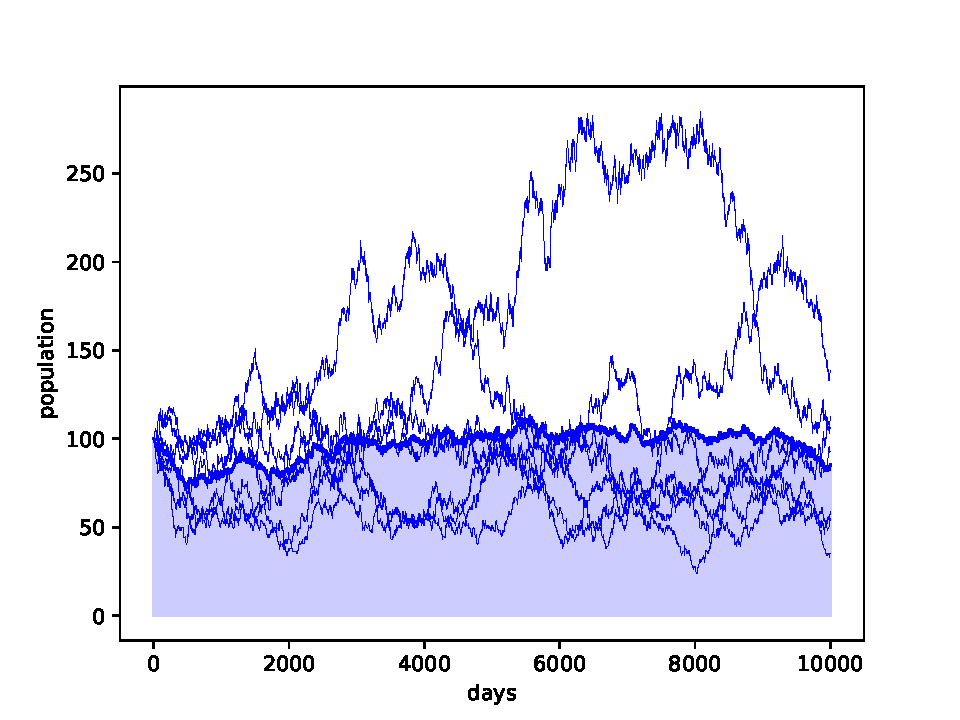
\includegraphics[width=\columnwidth]{figures/exp1_stable_pop}
        \caption{\textit{Exp 1:} Without any sort of tribe logic, the populations consists of solely \cowards.
        With some deviations, the population stays on average roughly the same at around \VNumPop.
        Visualized are \VNumSimulations random runs in light and their average in dark blue. }
        \label{fig:exp1_stable_pop}
    \end{figure}


    \subsubsection*{Experiment 2: General Altruism}

    We now analyze a more sophisticated way of survival by introducing concepts of collaboration and altruism.

    A first run shows that, as expected, introducing altruistic thinking leads to an increase in population size, visualized in \Cref{fig:exp2_total}.
    The population also reaches saturation pretty early on around day 1.500.

    \begin{figure}
        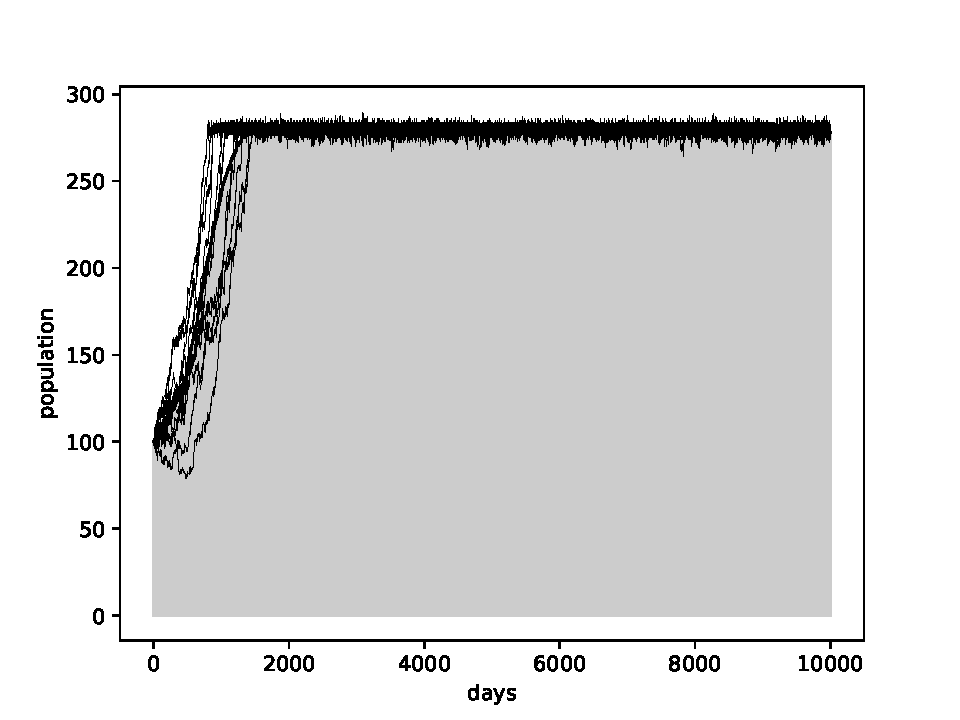
\includegraphics[width=\columnwidth]{figures/exp2_total}
        \caption{\textit{Exp 2:} As compared to the baseline case, introducing altruistic thinking leads to a big increase in and early saturation of population size.
        }
        \label{fig:exp2_total}
    \end{figure}

    We further analyze how this effect gets spread between the two types of agents.
    In \Cref{fig:exp2_sucker} we see that the amount of \suckers (aka altruists that help everyone) decreases steadily, while the population in general increases.
    This figure also shows that the amount of \cowards substantially increases.
    A potential explanation for this could be that in general the birth-rate for the \altruists is much lower than their die-off rate given their altruistic sacrifices.
    The cowards on the other hand, while having the same birth-rate, experience lower die-off-rates due to running away from a predator instead of helping.
    If we compare this to the original experiment without any altruism (\Cref{fig:exp1_stable_pop}), we see that this altruistic thinking has a large net-positive effect.
    This is the case even though the \suckers do not differentiate between whom they save.

    \begin{figure}
        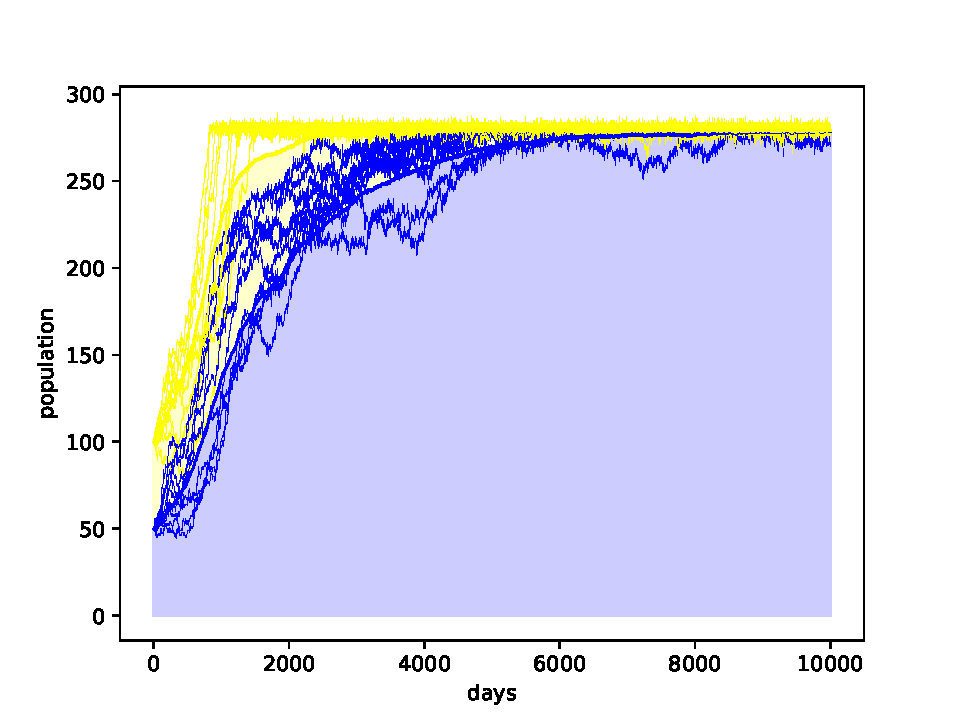
\includegraphics[width=\columnwidth]{figures/exp2_sucker}
        \caption{\textit{Exp 2:} Altruistic thinking leads to a large absolute increase in population.
        A saturation occurs around day 1.000, after which the increase in \cowards starts to slow down a little.
        By day 5.000 there are virtually no \suckers.}
        \label{fig:exp2_sucker}
    \end{figure}

    In the following \Cref{fig:exp2_sucker_rel} we see how these different types stack against each other when compared in relative terms.
    With a sharp increase right at the beginning, around $80\%$ of the population consists of cowards by day 2.500.
    While there are some runs where the \suckers were able to gain traction and constitute close to the majority at around day 1.000, by day 5.000 the population consists of 99\% \cowards with the \suckers going extinct in most runs.


    \begin{figure}
        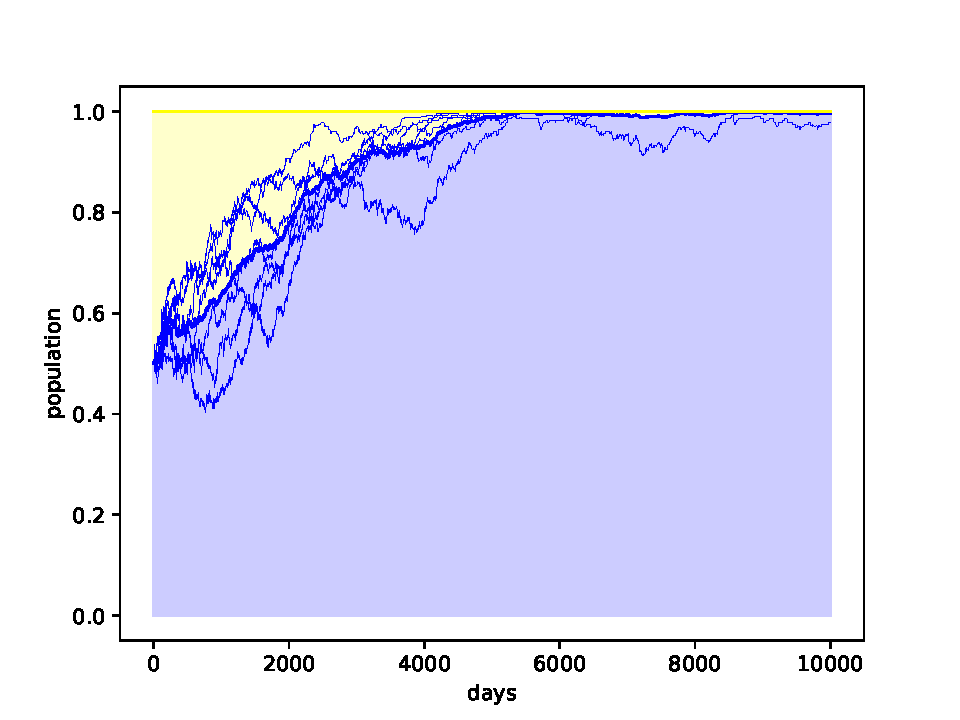
\includegraphics[width=\columnwidth]{figures/exp2_sucker_rel}
        \caption{\textit{Exp 2:} With altruistic thinking the proportion of \suckers declines linearly, reaching 0 after around 5.000 days on average.}
        \label{fig:exp2_sucker_rel}
    \end{figure}



    \subsubsection*{Experiment 3: Greenbeard Altruism}
    In the previous experiments we have seen that the \cowards experience an increase in population, while the \suckers/\altruists themselves do not benefit all too much (besides the net increase in general population).
    To fix this unfairness/inequality and to introduce another experiment, we consider the case where \altruists (here now \greenbeards) only help each other out.

    Looking at \Cref{fig:exp3_greenbeard}, we can see that our previously mentioned hypothesis is the case.
    The amount of \greenbeards increases substantially, while the number of \cowards drops equivalently, seemingly converging towards zero.
    We see that there is a general positive trend to be made out.
    This can further be seen in \Cref{fig:exp3_greenbeard_rel} where we have plotted the relative distribution of the different types.
    Interestingly enough, within the first 1.000 days, the number of \cowards seems to improve faster in relative and absolute terms.
    As soon as the population starts to saturate, the composition of the population shifts, with the proportion of \cowards reducing linearly.
    At day 2.000 the \greenbeards take up 50\% of the population, reaching 80\% at day 6.000 and 90\% by the end of day 10.000.



    \begin{figure}
        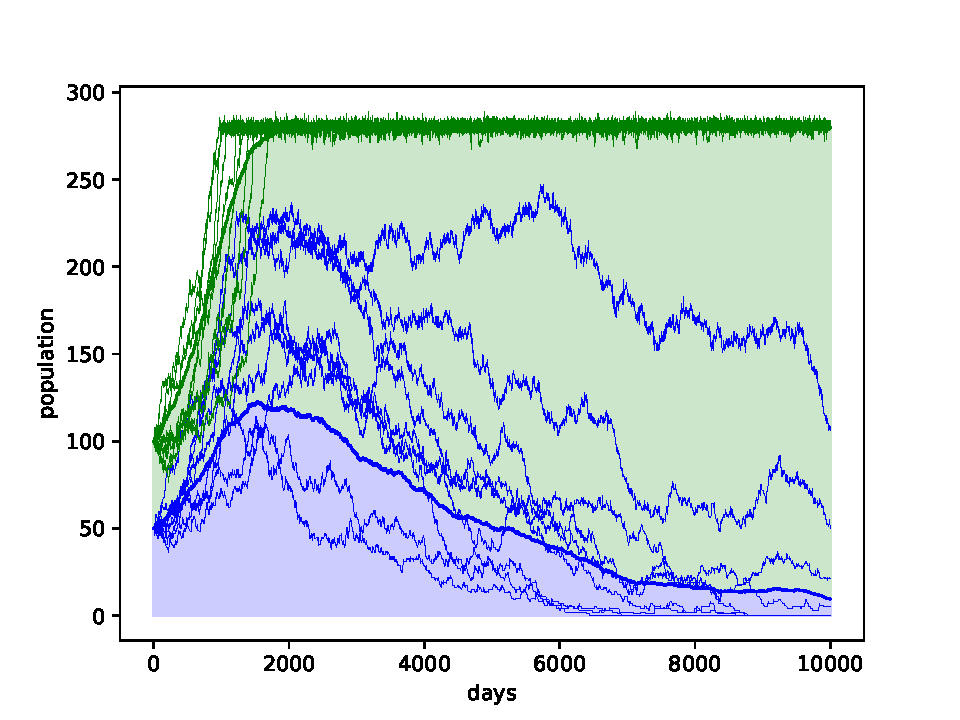
\includegraphics[width=\columnwidth]{figures/exp3_greenbeard}
        \caption{\textit{Exp 3:} When introducing \greenbeards that only help each other out, we see an increase in \cowards up until day 2.000 when the population saturates.
        After that the \greenbeards take over substantially.}
        \label{fig:exp3_greenbeard}
    \end{figure}


    \begin{figure}
        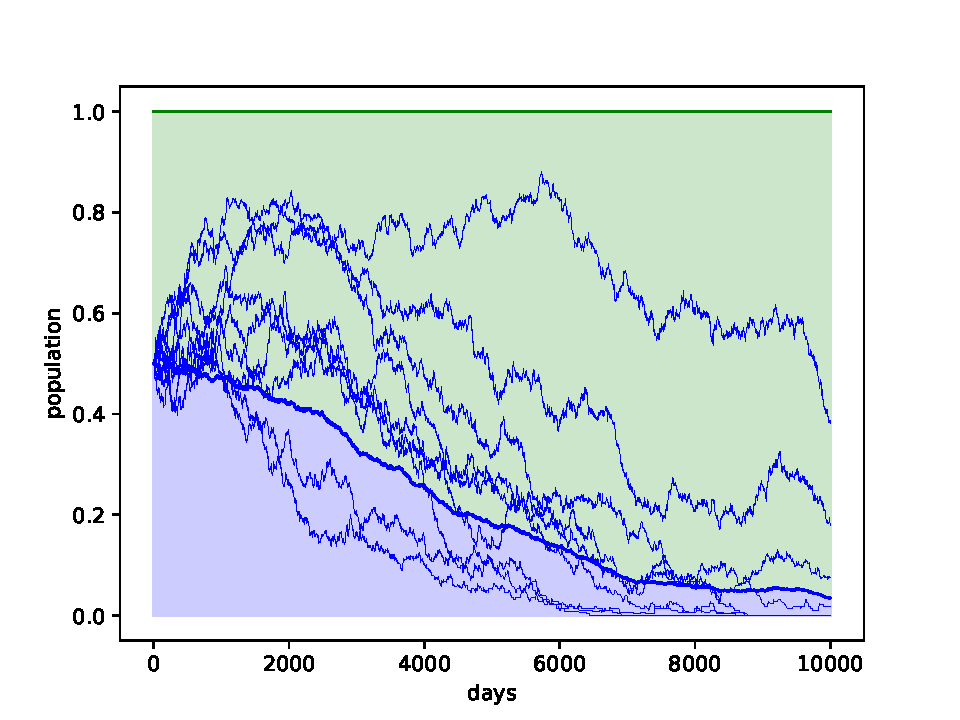
\includegraphics[width=\columnwidth]{figures/exp3_greenbeard_rel}
        \caption{\textit{Exp 3:} From a relative standpoint we see that the \greenbeard gene leads to a change in population composition.
        Constituting 42\% of the population at day 1.000 the \greenbeards end up at over 90\% by day 10.000.}
        \label{fig:exp3_greenbeard_rel}
    \end{figure}

    \subsubsection*{Experiment 4: On Trust and More}
    In our final experiment we run our simulations with all the previously mentioned tribes/types and add the notion of trust.
    We do this by introducing \impostors which to others appear as \greenbeards (allowing them to be rescued by other \greenbeards) but act as \cowards (not helping anyone) when they come across a difficult-job situation in both positions respectively.
    For the following plots we have omitted visualizing single runs for clarity.

    There are a few interesting insights that can be made out in such an environment.
    Looking at \Cref{fig:exp4_impostor} the first thing that can be noticed is that the population increases faster in the \coward-\greenbeard only case (\Cref{fig:exp3_greenbeard}) which saturates around day 2.000.
    Converging at around day 1.500, this experiment shows closer tendencies to the \coward-\sucker scenario (\Cref{fig:exp2_sucker}).

    Similarities to experiment 3 (\Cref{fig:exp3_greenbeard}) can still be made out in regard to the progression of the population types.
    As before, when the population saturates, the altruistic tribes see a downwards trend.
    At that point the amount of \impostors increases substantially while the \cowards can hold their own, decreasing only by around one third.

    Analyzing the relative frequencies in \Cref{fig:exp4_impostor_rel}, we see that the true altruists, the \suckers, are the first to go at around day 4.000.
    The \greenbeards, now being on their own against the non-altruists, are able to hold on until day 8.000 at which they also go extinct.
    After that, the proportion of \impostors and \cowards stays the same.
    This makes sense as without any \greenbeards the \impostors do not differ from simple \cowards.
    At the end the \impostors make up 80\% of the population while the \cowards take up 20 \%.

    This adds to the belief that such a \impostor genome offsets the benefits of \greenbeards holding together, supporting our first hypothesis (see \Cref{sec:hypothesis}) that misinformation has a major impact on the effectiveness of cooperation.

    In addition to the previously conducted experiment, we also wanted to explore whether different sized starting proportions of \impostors and \greenbeards allow a co-existence of cooperative behaviour in a dishonest society.
    Here, the share of \impostors resembles the amount of spread misinformation that results in distorted beliefs on other agents' behaviour/reputation.
    Keeping the sizes of \cowards and \suckers fixed, we vary the ratio of \greenbeards and \impostors.
    Since previous runs with equally sized starting shares of tribes/type showed that altruistic behaviour is doomed to go extinct, we wanted to give altruistic behaviour a second chance and thus varied the proportion of \impostors between 1\% and 25\%, resulting in runs with 1\%, 5\%, 10\%, and 25\% of \impostors at the beginning.
    The results of these simulations are visualized in \Cref{fig:misinformation}.

    Looking at these results, additional interesting trends can be made out.
    For instance, in three (\Cref{fig:misinformation} b, c, and d) out of four settings, altruistic behaviour always goes extinct or is about to die out soon.
    Only in one scenario (\Cref{fig:misinformation} a), where the proportion of \impostors starts out with 1\%, \greenbeards were sometimes capable to survive ($\sim 71\%$ of the runs) as \impostors went extinct by chance which explains the stagnation at around day 8.000.

    This provides evidence for our second hypothesis that as soon as misinformation gets introduced to the setting, altruism via cooperation gets unstable quickly and that the amount actually does not play a significant role.
    It is rather the case that \greenbeards can only survive if, in earlier stages of the simulations, \impostors go extinct by encountering too many faulty resources and do not receive help (encountering \cowards, or being the only one at a resource).

    Another interesting insight from these settings is the fact that altruistic behaviour seems to stick around longer depending on the initial proportion of \greenbeards but still goes extinct eventually.
    Furthermore, one final surprising observation can be made by looking at \Cref{fig:misinformation} a, i.e. a setting dominated by \greenbeards.
    In this case, green beard altruism showed its effectiveness again, similar to experiment 3 (\Cref{fig:exp3_greenbeard_rel}), where \cowards die out again in addition to \suckers.

    \begin{figure}
        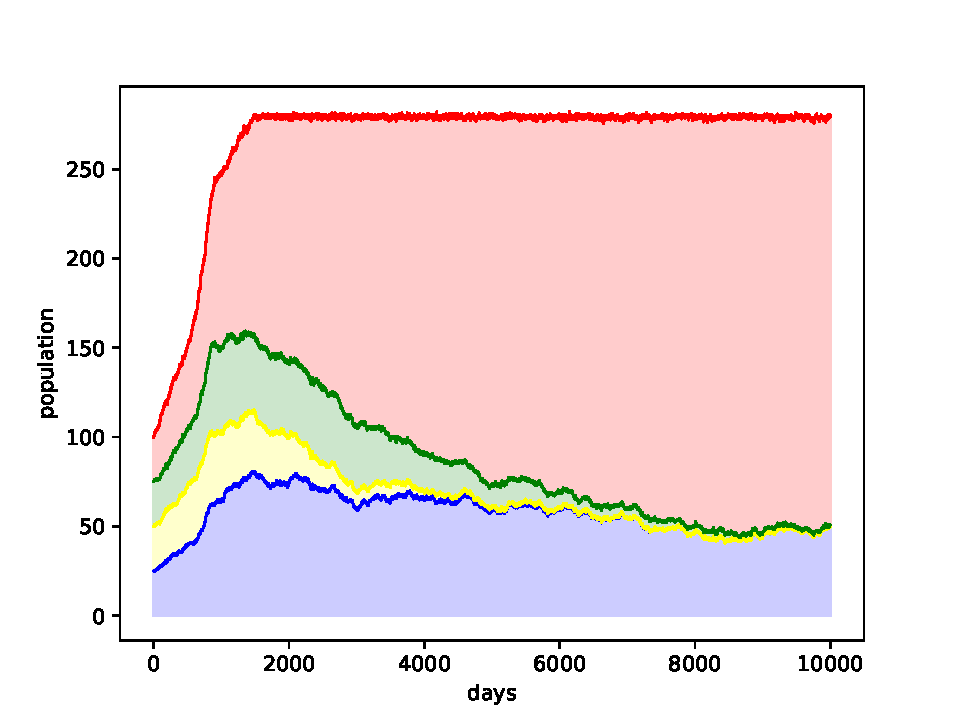
\includegraphics[width=\columnwidth]{figures/exp4_impostor}
        \caption{\textit{Exp 4:} The introduction of the \impostor genome in combination with all the other types leads to a faster population increase compared to the \coward-\greenbeard case in Experiment 3.}
        \label{fig:exp4_impostor}
    \end{figure}


    \begin{figure}
        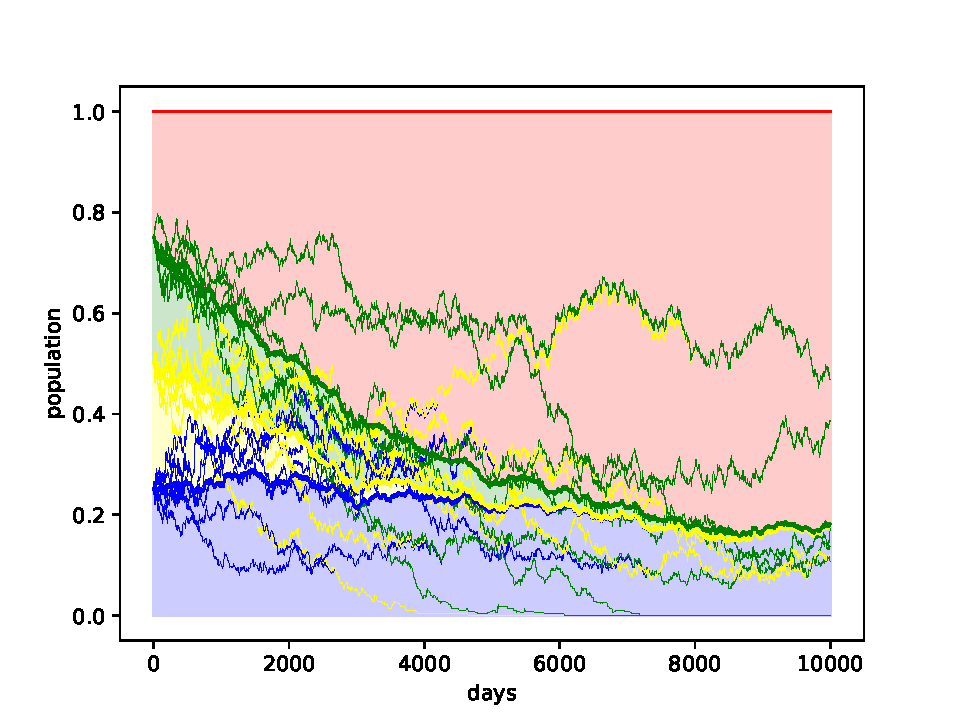
\includegraphics[width=\columnwidth]{figures/exp4_impostor_rel}
        \caption{\textit{Exp 4:} When looking at the relative frequencies of simulations encompassing all tribes, we see a large decrease in the altruistic types.
        On the other hand, \impostors increase linearly while the amount of \cowards only drops by around one third.
        Plotted is only the average of the simulations for brevity.}
        \label{fig:exp4_impostor_rel}
    \end{figure}

    \begin{figure*}
        \begin{subfigure}[b]{0.475\textwidth}
            \centering
            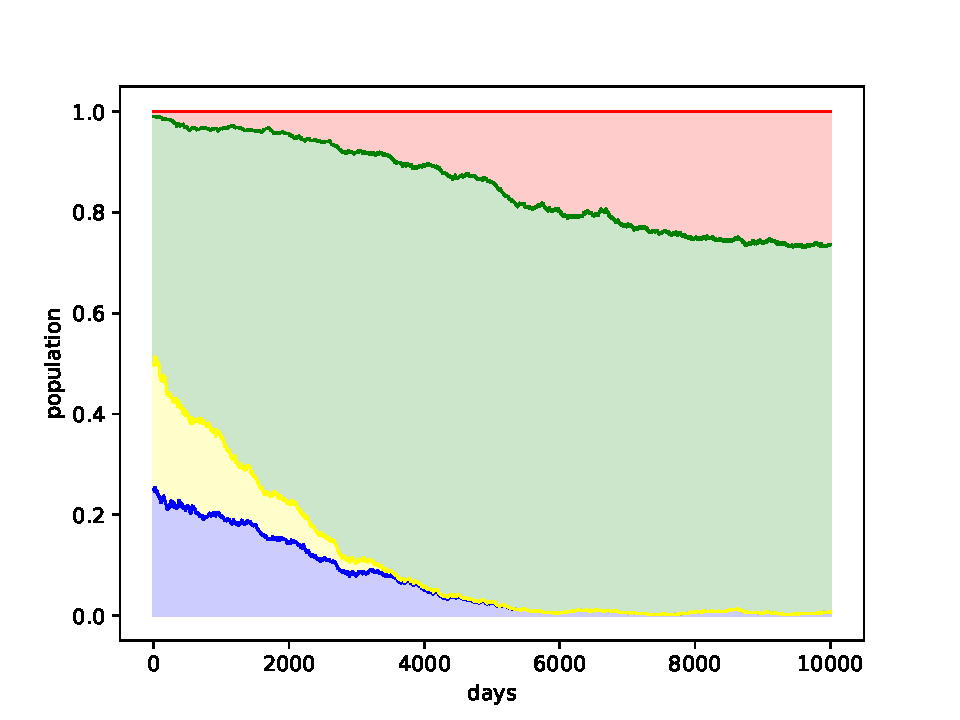
\includegraphics[width=\textwidth]{figures/exp4_impostor_1}
            \label{fig:1_imp}
            \caption{1\% \impostors (49\% \greenbeards)}
        \end{subfigure}
        \hfill
        \begin{subfigure}[b]{0.475\textwidth}
            \centering
            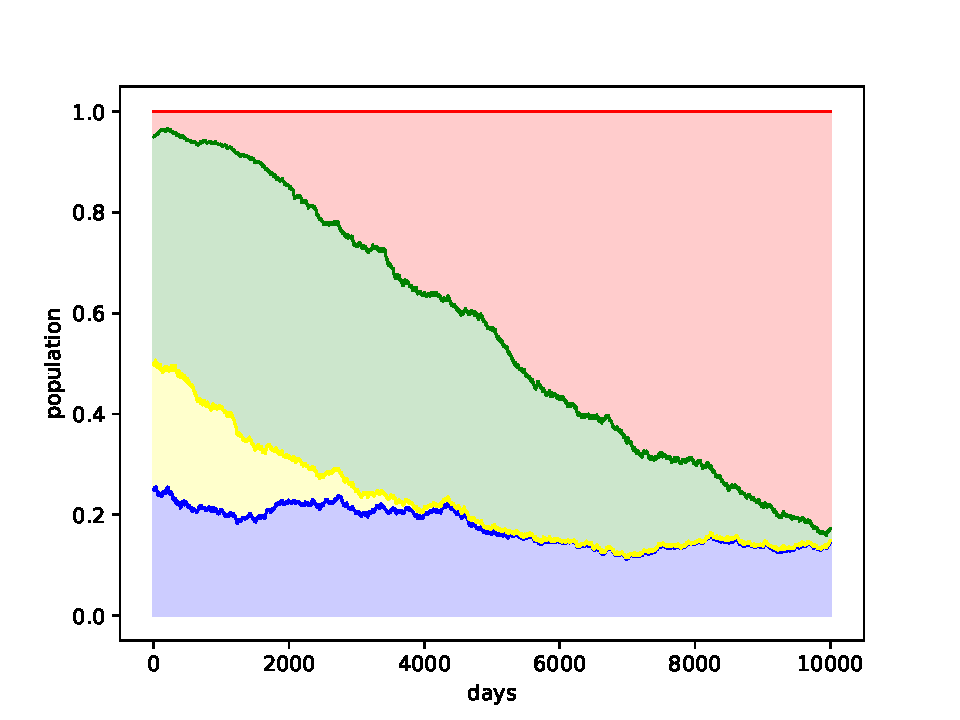
\includegraphics[width=\textwidth]{figures/exp4_impostor_5}
            \label{fig:5_imp}
            \caption{5\% \impostors (45\% \greenbeards)}
        \end{subfigure}
        \vskip\baselineskip
        \begin{subfigure}[b]{0.475\textwidth}
            \centering
            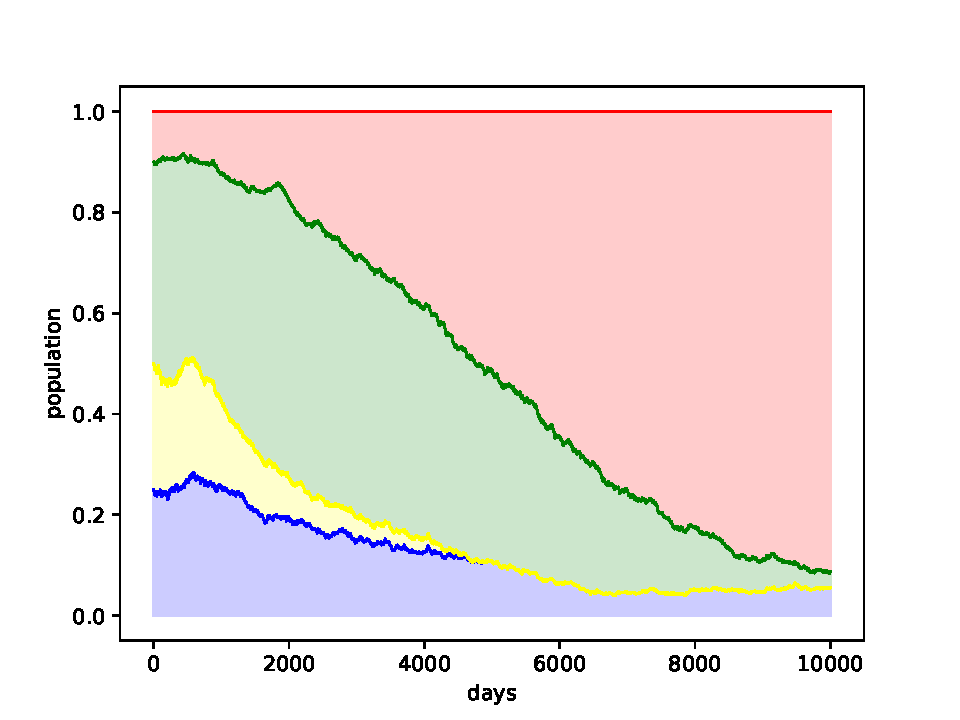
\includegraphics[width=\textwidth]{figures/exp4_impostor_10}
            \label{fig:10_imp}
            \caption{10\% \impostors (40\% \greenbeards)}
        \end{subfigure}
        \hfill
        \begin{subfigure}[b]{0.475\textwidth}
            \centering
            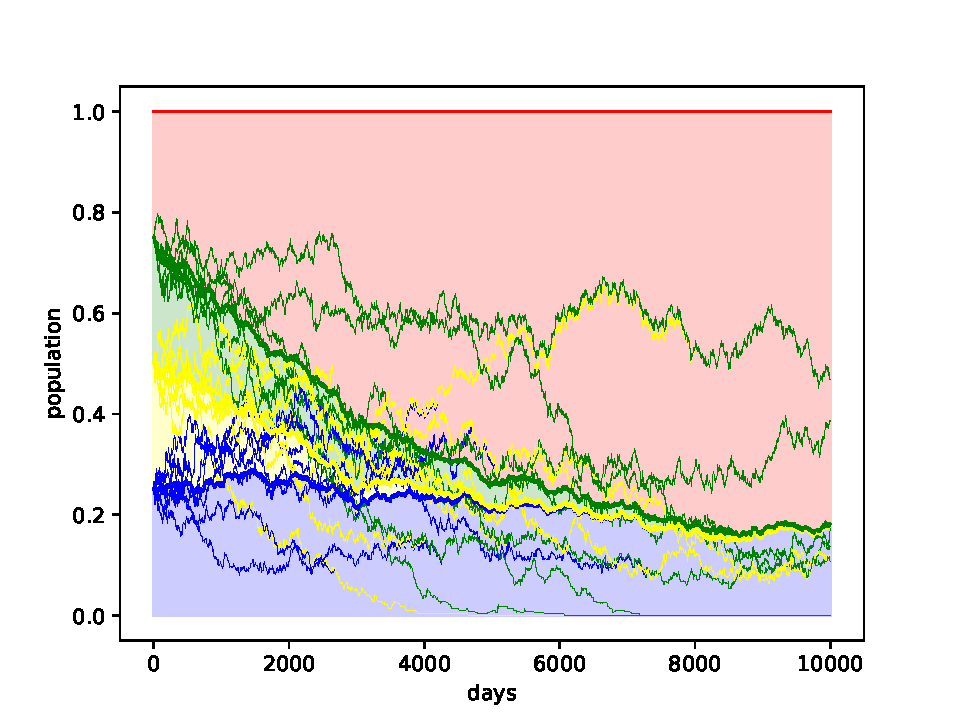
\includegraphics[width=\textwidth]{figures/exp4_impostor_rel}
            \label{fig:25_imp}
            \caption{25\% \impostors (25\% \greenbeards)}
        \end{subfigure}
        \caption{\textit{Exp 4:} Keeping the shares of \cowards and \suckers fixed, and only varying the ratio between \greenbeards and \impostors three interesting observations can be made: (i) in most of the runs altruistic behaviour goes extinct eventually with the exception of setting \textit{a}, (ii) a higher proportion of \greenbeards allows cooperative behaviour to survive longer, and (iii) in populations dominated by \greenbeards, \cowards die out again.
        }
        \label{fig:misinformation}
    \end{figure*}


    \section{Conclusion}\label{sec:conclusion}
    Based on the findings from our computer simulation, we empirically proved the correctness of our hypotheses, that is, (i) misinformation or deception has a major influence on the effectiveness of cooperation and (ii) the amount of misinformation does not necessarily play an important role rather if misinformation exists or not.
    We observed that altruism via reputation-based cooperation is a very unstable phenomenon which goes extinct in most of our simulations where \impostors, i.e. \textit{falsebeards}, are introduced.
    With these results, our work aligns well with the findings from \citeauthor{szamado_deception_2016} who conducted similar research to ours.
    Furthermore, we have showed that honesty and trust are key components for large-scale human societies to grow and exist.
    Only in setting where \greenbeards dominated the overall population and \impostors are almost non-existent, cooperation was sometimes still able to flourish.
    Lastly, in settings with just a small proportion of \impostors, \greenbeards and altruistic behaviour in general, were doomed to go extinct.
    Here, the introduction of punishment could be an effective countermeasure to maintain the correctness of someone's reputation which we leave open for future work.

    \bibliographystyle{ACM-Reference-Format}
    \bibliography{bibliography}

    \clearpage

    \onecolumn
    \section*{Appendix}

    \subsection{Experiment Configurations}\label{sec:configs}
    \subsubsection*{General Configuration}
    \lstinputlisting[language=Python,basicstyle=\tiny]{../core/config.py}

    \subsubsection*{Experiment 1}
    \lstinputlisting[language=Python,basicstyle=\tiny]{../core/experiments/exp1_stable_pop.py}

    \subsubsection*{Experiment 2}
    \lstinputlisting[language=Python,basicstyle=\tiny]{../core/experiments/exp2_cow_alt.py}

    \subsubsection*{Experiment 3}
    \lstinputlisting[language=Python,basicstyle=\tiny]{../core/experiments/exp3_greenbeard.py}

    \subsubsection*{Experiment 4}
    \lstinputlisting[language=Python,basicstyle=\tiny]{../core/experiments/exp4_impostor.py}

    \subsection{Code}\label{sec:code}
    \subsubsection*{Main}
    \lstinputlisting[language=Python,basicstyle=\tiny]{../main.py}

    \subsubsection*{Blob Class}
    \lstinputlisting[language=Python,basicstyle=\tiny]{../core/Blob.py}

    \subsubsection*{Method for Type-Specific Behaviour}
    \lstinputlisting[language=Python,basicstyle=\tiny]{../core/events/day.py}

    \subsubsection*{Method for Reproduction Mechanism}
    \lstinputlisting[language=Python,basicstyle=\tiny]{../core/events/night.py}

\end{document}
